\documentclass[12pt,a4paper]{report}  % ←ドキュメントクラスを追加
\usepackage[utf8]{inputenc}           % 文字コード指定
\usepackage{geometry}                 % 余白調整
\geometry{left=15mm,right=15mm,top=15mm,bottom=15mm}
\usepackage{url}
\usepackage{listings}

\usepackage{setspace}                 % 行間調整用
\usepackage{amsmath,amssymb}          % 数式用
% \usepackage{graphicx}                 % 画像を使う場合
\usepackage{titlesec}         
\usepackage[dvipdfmx]{graphicx} % 画像を使うためのパッケージ(日本語環境ならこれが無難)
\usepackage{here}          % 章タイトル調整
\usepackage{caption} % プリアンブルで追加
\lstnewenvironment{mylisting}[1][]
    {\lstset{
        frame=single,
        basicstyle=\ttfamily,
        numbers=left,
        numbersep=10pt,
        tabsize=2,
        extendedchars=true,
        xleftmargin=17pt,
        framexleftmargin=17pt,
        #1
    }
}{}
\renewcommand{\figurename}{図}
\renewcommand{\tablename}{表}

% --- 独自コマンド ---
\newcommand{\divergence}{\mathrm{div}\,}  % ダイバージェンス
\newcommand{\grad}{\mathrm{grad}\,}       % グラディエント
\newcommand{\rot}{\mathrm{rot}\,}         % ローテーション

% --- ページスタイル ---
\pagestyle{myheadings}

% --- タイトル情報 ---
\title{\Huge システムプログラミングII\\最終レポート}
\author{学生番号:5428 \\ 氏名:堀川風花}
\date{提出日:2025年1月21日}

\begin{document}

\maketitle    % ← タイトル(表紙)をここで出力!

% \setstretch{1.5}  % 行間を1.5倍に設定

\noindent
% レポート課題(11/11提出)\\[1em]  % ← [1em] は改行後の余白
\section{はじめに}
\subsubsection{目的}
\subsubsection{背景}

\section{サービスの概要}
本レポートでは以下のような構成のレンタルスペースの予約サービス(以下、本サービスという)を開発する。
本サービスでは会議室やパーティルームなどの「レンタルスペース」を、ユーザーがオンラインで予約できるサービスである。
管理者はレンタルスペースの登録や予約状況の確認などができる。
またレンタルスペースを予約した利用者は利用開始時刻の1時間前にGmailでリマインダーを受信する。

\begin{itemize}
  \item ユーザーの管理(認証、識別) \mbox{}\\
  本サービスを利用するユーザーを識別し、操作するための機能である。
  複数人でサービスを利用するため、ユーザーを追加したり、利用ユーザーを識別する機能が必要となる。
  \item レンタルスペースの管理(削除、編集、登録)\mbox{}\\
  レンタルスペースを予約する際には、まず予約する対象であるレンタルスペースを管理する必要がある。
  そのレンタルスペースの追加、削除できるようにする。
  \item レンタルスペースの予約の管理(キャンセル) 
  誰がそのレンタルスペースの予約をしているのかを管理する。
  \item リマインダー(Gmailに送信)
  利用開始時刻の1時間前に利用者のメールアドレスにGmailでリマインダーや
  サービスを提供できなくなった場合のキャンセルメール、
  利用が終了した際の感謝メールを送信する。
\end{itemize}


\section{システム構成}
\begin{center}
  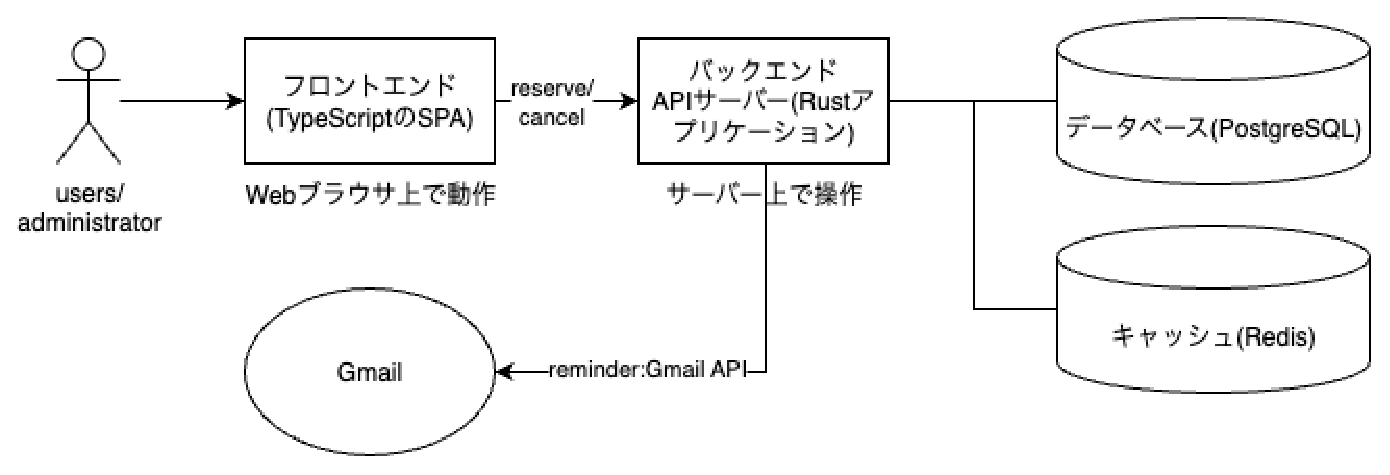
\includegraphics[width=0.7\linewidth]{/Users/horikawafuka2/Documents/class_2025/sp/reports/images/service2.eps}
  \captionof{figure}{サービス概要図}
  \label{fig:system_image}
\end{center}

\subsection{使用技術}
\begin{table}[h]
  \centering
\begin{tabular}{|l|r|} \hline
   分類& 使用技術  \\ \hline
   フロントエンド & TypeScript、React(Next.js) \\ \hline
   データベース &  PostgreSQL\\ \hline
   キャッシュ & Redis  \\ \hline
   バックエンド & Rust  \\ \hline
   サーバ & docker \\ \hline
   リマインダー & Gmail API\\ \hline
 \end{tabular}
   \caption{使用技術}
  \label{tb:use_module}
\end{table}

\subsection{モジュール構成}




\section{データベース設計}

データベース設計は図 \ref{fig:database_image}の通りである。

\begin{table}[h]
  \centering
\begin{tabular}{|l|r|} \hline
   データベース名& 内容  \\ \hline
   roles & \\ \hline
   users &  PostgreSQL\\ \hline
   spaces & Redis  \\ \hline
   resrvations & Rust  \\ \hline
   returned\_reservations & docker \\ \hline
 \end{tabular}
   \caption{使用技術}
  \label{tb:use_module}
\end{table}


\begin{center}
  \includegraphics[width=0.4\linewidth]{/Users/horikawafuka2/Documents/class_2025/sp/reports/images/database.eps}
  \captionof{figure}{データベース図}
  \label{fig:database_image}
\end{center}

\section{各種機能}
\subsection{利用者向け機能}
\subsubsection{ログイン機能}


\subsubsection{予約機能}



\subsubsection{予約確認機能}


\subsubsection{予約一覧表示機能}


\begin{center}
  \includegraphics[width=0.4\linewidth]{/Users/horikawafuka2/Documents/class_2025/sp/reports/images/eps/all_reservations_display.eps}
  \captionof{figure}{全ての予約の一覧画面}
  \label{fig:all_reservations_display_image}
\end{center}

\begin{center}
  \includegraphics[width=0.4\linewidth]{/Users/horikawafuka2/Documents/class_2025/sp/reports/images/eps/reservation_detail.eps}
  \captionof{figure}{予約の詳細画面}
  \label{fig:admin_reservation_detail_image}
\end{center}

\subsection{管理操作機能}
\subsubsection{予約サービス停止機能}


\subsubsection{予約キャンセル機能}



\subsubsection{スペース新規登録機能}


\subsubsection{スペース情報編集機能}



\subsubsection{スペース削除機能}


\subsection{通知機能}
\subsubsection{リマインドメール送信機能}


\subsubsection{キャンセルメール送信機能}


\subsection{加点対象機能}
\subsubsection{感謝メール送信機能}

\section{動作確認}
\subsection{動作確認環境}
動作環境は図 \ref{fig:dir}の通りである。
rusty-space-manegerがフロントエンドのコード、sp2025\_devが本体のサービスのコードである。

\begin{center}
  \includegraphics[width=0.2\linewidth]{/Users/horikawafuka2/Documents/class_2025/sp/reports/images/dir.eps}
  \captionof{figure}{ディレクトリ構造}
  \label{fig:dir}
\end{center}
ターミナルを二つ用いて実行させた。

\begin{mylisting}[language=c++,caption=ターミナル1のコマンド]
 sp2025_dev \%cargo make compose-remove 
 sp2025_dev \%cargo make build 
 sp2025_dev \%cargo make initial-setup 
 sp2025_dev \%cargo make run 
\end{mylisting}

\begin{mylisting}[language=c++,caption=ターミナル2のコマンド]
 rusty-space-maneger \%cd frontend/app
 app \% npm run dev
\end{mylisting}

管理者1人と利用者2人のアカウントを作成した。
\begin{table}[h]
  \centering
\begin{tabular}{|l|r|r|r|} \hline
   ユーザー名&権限&メールアドレス& パスワード  \\ \hline
   common user1& 利用者&m21137@g.metro-cit.ac.jp &password\\ \hline
   common user2&利用者& monariza0415@icloud.com& password\\ \hline
   admin user& 管理者&  horikawa0107tokyo@gmail.com &password \\ \hline
 \end{tabular}
   \caption{アカウント}
  \label{tb:account}
\end{table}


\subsection{利用者操作の動作確認手順}
\subsubsection{ログイン機能}
"http://localhost:3000"にアクセスし、メールアドレスとパスワードを入力する。
\begin{center}
  \includegraphics[width=0.4\linewidth]{/Users/horikawafuka2/Documents/class_2025/sp/reports/images/eps/login_page.eps}
  \captionof{figure}{ログイン画面}
  \label{fig:login_image}
\end{center}

\subsubsection{予約機能}
ログインすると図 \ref{fig:space_list_screen}の画面に遷移する。
\begin{center}
  \includegraphics[width=0.4\linewidth]{/Users/horikawafuka2/Documents/class_2025/sp/reports/images/eps/spaces_page.eps}
  \captionof{figure}{スペース一覧画面}
  \label{fig:space_list_screen}
\end{center}
スペースの中で、一つ選択するとスペースの詳細ページ(図 \ref{fig:space_detail_image})に移動する。

\begin{center}
  \includegraphics[width=0.4\linewidth]{/Users/horikawafuka2/Documents/class_2025/sp/reports/images/eps/space_table.eps}
  \captionof{figure}{スペースの詳細画面}
  \label{fig:space_detail_image}
\end{center}
左上の予約ボタンを押すと入力フォームが表示されるので希望の予約日時を指定し、"予約する"のボタンを押す。

\begin{center}
  \includegraphics[width=0.4\linewidth]{/Users/horikawafuka2/Documents/class_2025/sp/reports/images/eps/time_input.eps}
  \captionof{figure}{予約開始日時と予約終了日時を入力する画面}
  \label{fig:time_input_image}
\end{center}
指定した予約日時が予約日時帯が重複していたり、予約開始日時または、予約終了日時が現在時刻より前だった場合はエラーメッセージが表示される。
(図 \ref{fig:before_error_image}、図 \ref{fig:duplication_error_image}、図 \ref{fig:after_error_image})
\begin{center}
  \includegraphics[width=0.4\linewidth]{/Users/horikawafuka2/Documents/class_2025/sp/reports/images/eps/error_time_input1.eps}
  \captionof{figure}{予約開始日時が現在時刻より前だった場合のエラー}
  \label{fig:before_error_image}
\end{center}

\begin{center}
  \includegraphics[width=0.4\linewidth]{/Users/horikawafuka2/Documents/class_2025/sp/reports/images/eps/error_time_input2.eps}
  \captionof{figure}{予約日時帯が重複していた場合のエラー}
  \label{fig:duplication_error_image}
\end{center}

\begin{center}
  \includegraphics[width=0.4\linewidth]{/Users/horikawafuka2/Documents/class_2025/sp/reports/images/eps/error_time_input3.eps}
  \captionof{figure}{予約終了日時が現在時刻より前だった場合のエラー}
  \label{fig:after_error_image}
\end{center}
予約が成功すると成功アラートが表示される。(図\ref{fig:success_reserve_image})

\begin{center}
  \includegraphics[width=0.4\linewidth]{/Users/horikawafuka2/Documents/class_2025/sp/reports/images/eps/success_reserve.eps}
  \captionof{figure}{予約が成功した際のアラート}
  \label{fig:success_reserve_image}
\end{center}

\subsubsection{予約確認機能}
ヘッダー(図 \ref{fig:user_header})の”あなたの予約一覧”を選択する。
\begin{center}
  \includegraphics[width=0.4\linewidth]{/Users/horikawafuka2/Documents/class_2025/sp/reports/images/eps/user_header.eps}
  \captionof{figure}{利用者のヘッダー}
  \label{fig:user_header}
\end{center}
先ほどの予約が表示される。(図 \ref{fig:my_reservation_display_image})
\begin{center}
  \includegraphics[width=0.4\linewidth]{/Users/horikawafuka2/Documents/class_2025/sp/reports/images/eps/my_reservations_display.eps}
  \captionof{figure}{自分の予約一覧画面}
  \label{fig:my_reservation_display_image}
\end{center}

さらに押すと予約の詳細について確認できる。(図 \ref{fig:reservation_detail_image})

\begin{center}
  \includegraphics[width=0.4\linewidth]{/Users/horikawafuka2/Documents/class_2025/sp/reports/images/eps/reservation_detail.eps}
  \captionof{figure}{予約の詳細画面}
  \label{fig:reservation_detail_image}
\end{center}

また、個別の予約ごとにキャンセルが可能である。
\begin{center}
  \includegraphics[width=0.4\linewidth]{/Users/horikawafuka2/Documents/class_2025/sp/reports/images/eps/cancel_my_reservation.eps}
  \captionof{figure}{予約のキャンセルボタン(利用者)}
  \label{fig:cancel_my_reservation_button}
\end{center}


\subsection{管理者操作の動作確認手順}
利用者と同じようにログインする。

\subsubsection{全予約確認機能}
右上のヘッダーから"全ての予約一覧"を選択する。
\begin{center}
  \includegraphics[width=0.4\linewidth]{/Users/horikawafuka2/Documents/class_2025/sp/reports/images/eps/admin_header.eps}
  \captionof{figure}{管理者のヘッダー}
  \label{fig:admin_header}
\end{center}

全てのユーザの予約の一覧が表示される。

\begin{center}
  \includegraphics[width=0.4\linewidth]{/Users/horikawafuka2/Documents/class_2025/sp/reports/images/eps/all_reservations_display.eps}
  \captionof{figure}{全予約確認画面}
  \label{fig:all_reservations_list}
\end{center}

選択することで予約の詳細情報も閲覧できる。

\subsubsection{予約サービス停止機能}
左上の予約サービス停止ボタンを選択するとダイアログが現れ、再度確認を行う。
"停止する"を選択すると、全てのスペースが利用不可の状態となり予約は行えなくなる。

\begin{center}
  \includegraphics[width=0.4\linewidth]{/Users/horikawafuka2/Documents/class_2025/sp/reports/images/eps/stop_service.eps}
  \captionof{figure}{予約サービス停止ボタン}
  \label{fig:stop_reservation_service_dialog}
\end{center}

\begin{center}
  \includegraphics[width=0.4\linewidth]{/Users/horikawafuka2/Documents/class_2025/sp/reports/images/eps/success_stop_service.eps}
  \captionof{figure}{予約サービス停止機能が成功した場合のアラート}
  \label{fig:success_reservation_service_stop}
\end{center}

\begin{center}
  \includegraphics[width=0.4\linewidth]{/Users/horikawafuka2/Documents/class_2025/sp/reports/images/eps/success_stop_service.eps}
  \captionof{figure}{予約サービス停止機能が成功した場合のアラート}
  \label{fig:success_reservation_service_stop}
\end{center}

\subsubsection{予約キャンセル機能(管理者)}

\begin{center}
  \includegraphics[width=0.4\linewidth]{/Users/horikawafuka2/Documents/class_2025/sp/reports/images/eps/stop_service.eps}
  \captionof{figure}{予約サービス停止ボタン}
  \label{fig:stop_reservation_service_image}
\end{center}

\begin{center}
  \includegraphics[width=0.4\linewidth]{/Users/horikawafuka2/Documents/class_2025/sp/reports/images/eps/success_stop_service.eps}
  \captionof{figure}{予約サービス停止機能が成功しt場合のアラート}
  \label{fig:success_reservation_service_stop}
\end{center}
\subsubsection{スペース新規登録機能}

\begin{center}
  \includegraphics[width=0.4\linewidth]{/Users/horikawafuka2/Documents/class_2025/sp/reports/images/eps/space_info_input.eps}
  \captionof{figure}{新規登録用スペース情報入力画面}
  \label{fig:space_info_input_screen}
\end{center}

\subsubsection{スペース情報編集機能}

\begin{center}
  \includegraphics[width=0.4\linewidth]{/Users/horikawafuka2/Documents/class_2025/sp/reports/images/eps/space_edit_button.eps}
  \captionof{figure}{スペース情報編集ボタン}
  \label{fig:space_info_edit_button}
\end{center}

\begin{center}
  \includegraphics[width=0.4\linewidth]{/Users/horikawafuka2/Documents/class_2025/sp/reports/images/eps/change_is_active.eps}
  \captionof{figure}{スペース情報編集画面}
  \label{fig:change_is_active}
\end{center}
\subsubsection{スペース削除機能}
\begin{center}
  \includegraphics[width=0.4\linewidth]{/Users/horikawafuka2/Documents/class_2025/sp/reports/images/eps/delete_space_alert.eps}
  \captionof{figure}{スペース削除アラート}
  \label{fig:space_delete_alert}
\end{center}


\section{振り返り}
\section{まとめ}

\vskip\baselineskip











\vskip\baselineskip

\subsubsection{グループの傾向}
\begin{itemize}
\item グループ1 \mbox{}\\
複数のトピックが共通しており、トピックの内容は地域や教育関係と
広い範囲にわたる。地域行政や学校教育を重視する傾向がある。

\item グループ2 \mbox{}\\
教育・学校・教育\_委員などの教育行政のトピックが強いエッジで重なっており、
教育関係と教育を受ける子供を重視する傾向がある。 
\item グループ3 \mbox{}\\
発電・エネルギー・電力などインフラ関係やエネルギー政策に関心があることが見てとれる。
  \end{itemize}

\vskip\baselineskip



% \begin{center}
%   \includegraphics[width=0.7\linewidth]{/Users/horikawafuka2/Documents/class_2025/dm/後期中間/reports/images/700_speakers_cc_network_colored.eps}
%   \captionof{figure}{グループ分けした共起ネットワーク(議員24人)}
% \end{center}


\section{参考文献}
% 参考文献を強制改ページしない設定
\begingroup
\renewcommand{\chapter}[2]{} % chapterとして認識させない
\begin{thebibliography}{2}
\bibitem{word cloud} Non."【簡単】Pythonでワードクラウドを作る方法".note.20243-09-13,\url{https://note.com/noa813/n/n777ba133e62f},(2025-10-28)
\bibitem{cc network} osn Lofi."【自然言語処理】【Python】共起ネットワークの作り方を理解する".Zenn.2022-10-08,\url{https://zenn.dev/robes/articles/a3e1a6e80efd99},(2025-10-29)
\bibitem{masuzoe yoichi} 公明党."都市外交を積極的に".公明党公式ホームページ.2014-03-05,\url{https://www.komei.or.jp/news/detail/20140305_13423},(2025-11-03)

\end{thebibliography}
\endgroup

\end{document}